\documentclass{beamer}
\usepackage[utf8]{inputenc}
\usepackage[spanish]{babel}
\usepackage{hyperref}
\usepackage{verbatim}
\usepackage{listings}

\setbeamercovered{invisible}
\usetheme{Frankfurt}
\usefonttheme{serif}

% Configurar los listings (Códigos)
\renewcommand{\lstlistingname}{Código}
\lstset{
	language=C++,               % Lenguaje
	basicstyle=\ttfamily\footnotesize,  % Tipo de fuente
	keywordstyle=\color{blue},  % Color de palabras clave
	stringstyle=\color{red},    % Color de strings
	commentstyle=\color{gray},  % Color de comentarios
	showstringspaces=false,     % No muestrar el _ cuando el string tiene espacios
	breaklines = true,          % Partir las líneas largas
	breakatwhitespace=true,	    % Partir las líneas en un espacio
	numbers=left,				% Numerar las líneas a la izq
	numberstyle=\tiny,			% Poner los números de las líneas pequeños
	numberblanklines=true,      % Numerar las líneas en blanco
	columns=fullflexible,       % No perder el formato al dejar los espacios
	keepspaces=true,   			% Dejar los espacios insertados
	frame=tb,					% Poner el recuadro
}

\AtBeginSection[]{%
  \begin{frame}<beamer>
    \frametitle{Contenido}
    \tableofcontents[sectionstyle=show/hide,subsectionstyle=hide/show/hide]
  \end{frame}
  \addtocounter{framenumber}{-1}% If you don't want them to affect the slide number
}

\title{Semillero de Programación}
\subtitle{Ordenamiento Topológico, Componentes Fuertemente Conexas y Estructuras de Datos}
\author{Ana Echavarría \and Juan Francisco Cardona}

\institute{Universidad EAFIT}
\date{8 de marzo de 2013}

\begin{document}

\begin{frame}
	\titlepage
\end{frame}

\begin{frame}
	\frametitle{Contenido}
	\tableofcontents
\end{frame}

\section{Ordenamiento Topológico}
	\begin{frame}
		\frametitle{DAG}
		\begin{block}{DAG}
			Un DAG (Directed Acyclic Graph) es un grafo dirigido que no tiene ciclos.
		\end{block}
		\begin{center} 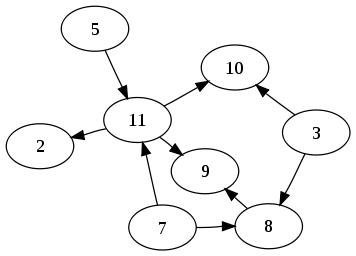
\includegraphics[height = 0.4\textheight]{DAG.png} \end{center}
	\end{frame}
	
	\begin{frame}
		\frametitle{Ordenamiento Topológico}
		\begin{block}{Ordenamiento Topológico}
			Un ordenamiento topológico o topological sort de un DAG $G = (V, E)$ es un ordenamiento lineal de sus nodos $V$ de tal forma que si $(u, v) \in E$ entonces $u$ aparece antes que $v$ en el ordenamiento.\\
			Este ordenamiento se puede ver como una forma de poner todos los nodos en una línea recta y que las aristas vayan todas de izquierda a derecha.
		\end{block}
	\end{frame}
	
	\begin{frame}
		\frametitle{Ejemplo}
		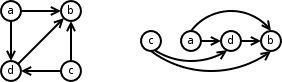
\includegraphics[width = 0.95\textwidth]{toposort.png}
	\end{frame}
	
	\begin{frame}
		\frametitle{Algoritmo}
		\begin{enumerate}
			\item Hacer un DFS con el grafo
			\item Cuando marco un nodo como negro, lo inserto a un vector
			\item Reversar el orden de los elementos del vector
			\item El vector contiene un ordenamiento topológico del grafo
		\end{enumerate}
	\end{frame}
	
	\begin{frame}[fragile]
		\frametitle{Algoritmo}
		\begin{lstlisting}
			vector <int> g[MAXN];
			bool seen[MAXN];
			vector <int> topo_sort;

			void dfs(int u){
			   seen[u] = true;
			   for (int i = 0; i < g[u].size(); ++i){
			      int v = g[u][i];
			      if (!seen[v]) dfs(v);
			   }
			   topo_sort.push_back(u); // Agregar el nodo al vector
			}
			int main(){
			   // Build graph: n = verices 
			   topo_sort.clear();
			   for (int i = 0; i < n; ++i) seen[i] = false;   
			   for (int i = 0; i < n; ++i) if (!seen[i]) dfs(i);  
			   reverse(topo_sort.begin(), topo_sort.end());
			   return 0;
			}
		\end{lstlisting}
	\end{frame}
	
	\begin{frame}
		\frametitle{Ejemplo}
		\begin{center} 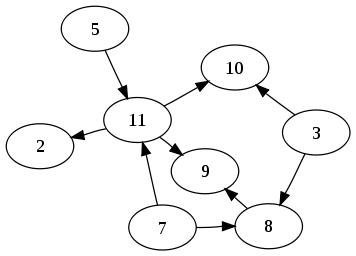
\includegraphics[height = 0.7\textheight]{DAG.png} \end{center}
	\end{frame}
	
	\begin{frame}
		\frametitle{¿Por qué funciona?}
		\begin{itemize}
			\item Cuando se inserta un nodo a la lista, es porque ya procesé todos sus vecinos.
			\item Si ya procesé todos sus vecinos, ellos ya están en la lista.
			\item Cuando meto un nodo a la lista, todos sus vecinos ya están antes que él en la lista, entonces en el ordenamiento van a quedar después de él.
			\item En conclusión, en el ordenamiento que generamos, los vecinos de cada nodo van a estar después de él por lo que es un ordenamiento topológico.
		\end{itemize}
	\end{frame}
	
	\begin{frame}
		\frametitle{Complejidad}
		\begin{block}{Complejidad}
			Hacer el ordenamiento topológico toma $O(V+E)$ para el dfs y $O(V)$ para reversar la lista. En total la complejidad es $O(V+E)$.
		\end{block}
	\end{frame}


\section{Componentes Fuertemente Conexas}
	\begin{frame}
		\frametitle{Componentes Fuertemente Conexas}
		\begin{block}{SCC}
			Dado un grafo dirigido $G = (V, E)$, un componente fuertemente conexa o strongly connected component (SCC) de $G$ es un subconjunto $C$ de nodos que cumple que para cada pareja $u, v \in C$ existe un camino de $u$ a $v$ y de $v$ a $u$ y que $C$ es lo más grande posible. 
		\end{block}
		\begin{center} 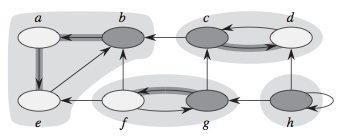
\includegraphics[height = 0.3\textheight]{scc.png} \end{center}
	\end{frame}
	
	\begin{frame}
		\frametitle{Algoritmo}
		\begin{enumerate}
			\item Crear el grafo $G$ y el grafo $G_{rev}$ que es el mismo que $G$ pero con las aristas invertidas.
			\item Hacer DFS en el grafo G y generar su ``ordenamiento topológico'' (incluir un nodo a la lista solo cuando haya visto todos los nodos alcanzables desde él.)
			\item Hacer un DFS en el grafo reversado $G_{rev}$ pero hacer las llamadas en el orden del ``ordenamiento topológico''.
			\item Cada llamado a este último DFS halla una componente fuertemente conexa.
		\end{enumerate}
	\end{frame}
	
	\begin{frame}
		\frametitle{Ejemplo}
		\begin{center} 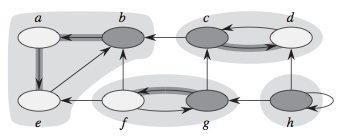
\includegraphics[height = 0.5\textheight]{scc.png} \end{center}
	\end{frame}
	
	\begin{frame}[allowframebreaks]
		\frametitle{¿Por qué funciona?}
		\begin{enumerate}
			\item Las componentes fuertemente conexas de $G$ son las mismas que las de $G_{rev}$.
			\item Si comprimo los nodos de una misma componente en un solo nodo, quedo con un DAG.
			\item Si tengo dos componentes distintas $C_1$ y $C_2$ de manera que haya una arista de un nodo de $C_1$ a un nodo de $C_2$, entonces todos los nodos de $C_1$ van a quedar después que los nodos de $C_2$ en el ``ordenamiento topológico'' que se hace con el primer DFS.
			\framebreak
			\item Los nodos que quedan de primeros en el ``ordenamiento topológico'' son los nodos de una componente $C$ a la cual no llega ninguna arista.
			\item En el grafo $G_{rev}$, de la componente $C$ no sale ninguna arista.
			\item Cuando llamo el segundo DFS lo hago desde $C$ y sólo descubro los elementos de $C$.
			\item Cuando llamo el segundo DFS desde otro nodo este puede no tener aristas salientes o tener aristas salientes a $C$ pero como ya descubrí todo en $C$ sólo voy a descubrir lo que hay en la componente de ese nodo
		\end{enumerate}
	\end{frame}

\section{Dominos}
	\begin{frame}
		\frametitle{Problema 11504 - Dominos}
		\begin{block}{Problema}
			Hallar el mínimo número de dominós que hay que derribar a mano para que todos los dominós se derriben.
		\end{block}
	\end{frame}
	
	\begin{frame}
		\frametitle{Ideas}
		\begin{alertblock}{Ideas}
			\begin{itemize}
				\item ¿Qué pasa con las cadenas de dominós que forman un ciclo? ¿Cuántos necesito máximo para derribarlas? \pause
				\item ¿Puedo entonces considerar los ciclos como un sólo dominó? ¿Qué algoritmo estoy utilizando? \pause
				\item En el grafo que se forma cuando junto los elementos de las mismas componentes ¿cuántos dominós tengo que derribar?
			\end{itemize}
		\end{alertblock}
	\end{frame}
	
	\begin{frame}
		\frametitle{Solución}
		\begin{enumerate}
			\item Crear el grafo dirigido y su grafo invertido
			\item Hallar la componente fuertemente conexa de cada nodo
			\item Hallar cuántas aristas llegan a cada componente conexa
			\item Contar cuántas componentes hay a las cuales no lleguen aristas
		\end{enumerate}
	\end{frame}
	
	\begin{frame}[fragile]
		\frametitle{Variables globales}
		\begin{lstlisting}
			// El maximo numero de dominos
			const int MAXN = 100005; 
			// El grafo
			vector <int> g[MAXN];
			// El grafo reversado    
			vector <int> grev[MAXN];
			// El "ordenamiento topologico" del grafo G 
			vector <int> topo_sort;  
			// La componente fuertemente conexa a la que pertenece cada nodo
			int scc[MAXN];  
			// El arreglo de visitado para el primer DFS         
			bool seen[MAXN];
			 // El numero de aristas entrantes a cada componente         
			int in[MAXN];           
		\end{lstlisting}
	\end{frame}
	
	\begin{frame}[fragile]
		\frametitle{DFS}
		\begin{lstlisting}
			// DFS donde se halla el ordenamiento topologico
			void dfs1(int u){ 
			   seen[u] = true;
			   for (int i = 0; i < g[u].size(); ++i){
			      int v = g[u][i];
			      if (!seen[v]) dfs1(v);
			   }
			   topo_sort.push_back(u);
			}
			// DFS donde se hallan las componentes
			void dfs2(int u, int comp){ 
			   scc[u] = comp;
			   for (int i = 0; i < grev[u].size(); ++i){
			      int v = grev[u][i];
			      if (scc[v] == -1) dfs2(v, comp);
			   }
			}
		\end{lstlisting}
	\end{frame}
	
	\begin{frame}[fragile, allowframebreaks]
		\frametitle{Main}
		\begin{lstlisting}
			int main(){
			   int cases; cin >> cases;
			   while (cases--){
			      int n, m;
			      cin >> n >> m;
			
			      // Limpiar las variables entre caso y caso
			      for (int i = 0; i <= n; ++i){
			         g[i].clear();
			         grev[i].clear();
			         topo_sort.clear();
			         scc[i] = -1;
			         seen[i] = false;
			         in[i] = 0;
			      }
			
			
			
			      // Crear el grafo y el grafo reversado
			      for (int i = 0; i < m; ++i){
			         int u, v; cin >> u >> v;
			         u--; v--;
			         g[u].push_back(v);
			         grev[v].push_back(u);
			      }
			
			      // Llamar el primer dfs
			      for (int i = 0; i < n; ++i){
			         if (!seen[i]) dfs1(i);
			      }
			      reverse(topo_sort.begin(), topo_sort.end()); 
			      // Llamar el segundo dfs
			      int comp = 0;
			      for (int i = 0; i < n; ++i){
			         int u = topo_sort[i];
			         if (scc[u] == -1) dfs2(u, comp++);
			      }
			
			      // Ver cuantas aristas entrantes tiene cada componente
			      for (int u = 0; u < n; ++u){
			         for (int i = 0; i < g[u].size(); ++i){
			            int v = g[u][i];
			            if (scc[u] != scc[v]) in[scc[v]]++;
			         }
			      }
			
			      // Sumar las componentes que tienen 0 aristas entrantes
			      int count = 0;
			      for (int u = 0; u < comp; ++u){
			         if (in[u] == 0) count++;
			      }
			      cout << count << endl;
			   }
			    return 0;
			}
		\end{lstlisting}
	\end{frame}

\section{Map}
	\begin{frame}[fragile]
		\frametitle{Map}
		\begin{block}{Map}
			Un mapa es un contenedor que guarda parejas de elementos. El primer elemento de la pareja (key) sirve para identificarla y el segundo elemento (mapped value) es el valor asociado a la llave.\\
		\end{block}
		\begin{block}{Declaración}
			\verb|#include <map>|\\
			\verb|map <tipo_dato_key, tipo_dato_value> nombre;|\\
			Ejemplos:\\
			\verb|map <string, int> m;|\\
			\verb|map <char, int> char2int;|
		\end{block}
	\end{frame}
	
	\begin{frame}[fragile]
		\frametitle{Acceso a elementos de un mapa}
		Los elementos de un mapa se llaman por su llave así:\\ \quad \\
		\verb|map <string, int> m;|\\
		\verb|m["Hola"] = 3;|\\
		\verb|int a = m["Cangrejo"];|\\ \quad \\
		
		Para ingresar un elemento se puede hacer así:\\
		\verb|if (m.count["Nuevo"] == 0) m["Nuevo"] = 123;|\\ \quad \\
		Con la función \verb|count| se busca cuántas veces está el elemento con la llave \verb|"Nuevo"|. Si el elemento no está, cuando accedemos a él con \verb|[]| éste se crea automáticamente.\\
		Cuando accedo con \verb|[]| a un elemento del mapa que no existe este se crea con valores por defecto. Para strings es el string vacío \verb|""| y para enteros es el número 0.
	\end{frame}
	
	\begin{frame}
		\frametitle{Complejidad del mapa}
		\begin{block}{Complejidad}
			\begin{itemize}
				\item Insertar / acceder un elemento al mapa es $O(log\,n \times k)$ donde $n$ es el número de elementos en el mapa y $k$ es el tiempo que toma comparar dos llaves del mapa.
				\item Comparar dos enteros es $O(1)$, comparar dos strings es $O(m)$ donde $m$ es la longitud de los strings.
				\item Insertar / acceder un elemento a un mapa con llaves strings es $O(log\,n \times m)$ donde $n$ son los elementos del mapa y $m$ es la longitud del string.
			\end{itemize}
		\end{block}
		\begin{block}{Nota}
			Los elementos de un mapa se almacenan en orden de acuerdo a una función de comparación. Por defecto la función de comparación es la de menor, es decir que los elementos se almacenan de menor a mayor.
		\end{block}
	\end{frame}
	
	\begin{frame}[fragile]
		\frametitle{Recorrer un mapa}
		Para recorrer un mapa es necesario usar iteradores.\\
		\begin{lstlisting}
		#include <iostream>
		#include <map>
		using namespace std;

		int main(){
		   map <string, int> m;
		   m["b"] = 4;
		   m["bc"] = 1;
		   m["a"] = 3;
		   map <string, int> :: iterator it;
		   for (it = m.begin(); it != m.end(); it++){
		      cout << "( " << it->first << " " << it->second << " ) ";
		      // cout << "( " << (*it).first << " " << (*it).second << " ) ";
		   }
		   return 0;
		}
		// La funcion imprime ( a 3 ) ( b 4 ) ( bc 1 )
		\end{lstlisting}
	\end{frame}
	
	\begin{frame}[fragile]
		\frametitle{Otras funciones en el mapa}
		Otras funciones que se pueden hacer con el mapa son:\\
		\begin{itemize}
			\item Recorrerlo al revés con \verb|rbegin| y \verb|rend|
			\item Obtener el tamaño con \verb|size|
			\item Borrar el contenido con \verb|clear|
			\item Insertar elementos (si no están antes) con \verb|emplace|
			\item Borrar elementos con \verb|erase|
			\item Buscar un elemento con \verb|find|
		\end{itemize}
		\quad \\
		Para más información mirar \url{http://www.cplusplus.com/reference/map/map/}
	\end{frame}
	
	\section{Set}
	\begin{frame}[fragile]
		\frametitle{Set}
		\begin{block}{Set}
			Un set es un contenedor que guarda conjuntos, es decir grupos de elementos iguales donde cada elemento aparece una sola vez.\\
			Los elementos de un set se almacenan en orden de acuerdo a una función de comparación. Por defecto la función de comparación es la de menor, es decir que los elementos se almacenan de menor a mayor.\\
		\end{block}
		\begin{block}{Declaración}
			\verb|#include <set>|\\
			\verb|set <tipo_dato> nombre;|\\
			Ejemplos:\\
			\verb|set <string> s;|\\
			\verb|set <int> amigos;|
		\end{block}
	\end{frame}

	\begin{frame}[fragile]
		\frametitle{Operaciones sobre un set}
		Sobre un set se pueden hacer las siguientes operaciones.
		\begin{description}
			\item[insert] Inserta un elemento al set. Ejemplo: \verb|amigos.insert(9)|
			\item[count] Cuenta cuántas veces aparece un elemento (0 o 1 vez). Ejemplo: \verb|amigos.count(3)|
			\item[find] Retorna un iterador al lugar donde está el elemento. Ejemplo: \verb|amigos.find(3)|
			\item[erase] Elimina un elemento del set. Ejemplo: \verb|amigos.erase(amigos.find(3))|
		\end{description}
		Todas las operaciones anteriores tienen una complejidad $O(log\,n \times k)$ donde $n$ es el número de elementos del set y $k$ es el tiempo que toma comparar dos elementos.\\
		Para más información mirar \url{http://www.cplusplus.com/reference/set/set/}
	\end{frame}

	\begin{frame}[fragile]
		\frametitle{Recorrer un set}
		Para recorrer un set es necesario usar iteradores.\\
		\begin{lstlisting}
		#include <iostream>
		#include <set>
		using namespace std;

		int main(){
		   set <int> s;
		   s.insert(4); 
		   s.insert(-1);
		   s.insert(3);
		   s.insert(4);
		   set <int> :: iterator it;
		   for (it = s.begin(); it != s.end(); it++){
		      cout << *it << " ";
		   }
		   return 0;
		}
		// La funcion imprime -1 3 4
		\end{lstlisting}
	\end{frame}
	
\section{Heap}
	\begin{frame}
		\frametitle{Heap}
		\begin{block}{Heap}
			Un heap es una estructura de datos en forma de árbol binario en la que cada padre tiene un valor mayor o igual al de sus dos hijos
		\end{block}
		\begin{center}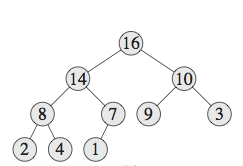
\includegraphics[height = 0.5\textheight]{heap.png} \end{center}
	\end{frame}
	
	\begin{frame}
		\frametitle{¿Cómo funciona la inserción en un heap?}
		\begin{columns}
			\column{0.33\textwidth}
			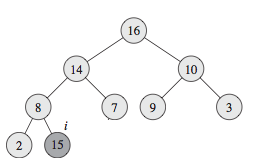
\includegraphics[width = 1.15\textwidth]{heap_insert1.png}
			\column{0.33\textwidth}
			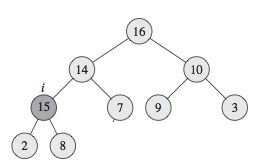
\includegraphics[width = 1.15\textwidth]{heap_insert2.png}
			\column{0.33\textwidth}
			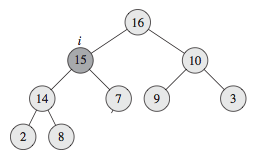
\includegraphics[width = 1.15\textwidth]{heap_insert3.png}
		\end{columns}
	\end{frame}
	
	\begin{frame}
		\frametitle{¿Cómo funciona la extracción en un heap?}
		\begin{columns}
			\column{0.5\textwidth}
			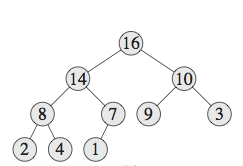
\includegraphics[width = 1\textwidth]{heap.png}
			\column{0.5\textwidth}
			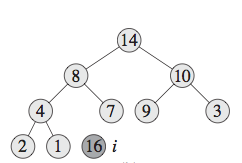
\includegraphics[width = 1\textwidth]{heap_delete.png}
		\end{columns}
	\end{frame}
	
	
	\begin{frame}[fragile]
		\frametitle{Representación en C++}
		Un heap se puede representar en C++ como una cola de prioridades así:
		\verb|#include <queue>|\\
		\verb|priority_queue <tipo_dato> nombre;|\\
		Ejemplos:\\
		\verb|priority_queue <int> heap;|\\
		\verb|priority_queue <pair <int, int> > q;|\\
		\quad \\
		Para más información mirar: \url{http://www.cplusplus.com/reference/queue/priority_queue/}
	\end{frame}
	
	
	\begin{frame}
		\frametitle{Operaciones}
		La cola de prioridades (heap) soporta las siguientes operaciones
		\begin{description}
			\item [push] Inserta un elemento
			\item [pop] Extrae un elemento
			\item [top] Retorna el máximo elemento de la cola (heap)
			\item [size] Retorna el tamaño de la cola (heap)
		\end{description}
		\quad \\
		La cola de prioridades se ordena de acuerdo a la función de ordenamiento $<$ (menor que) por lo que retorna el elemento con el cual todos los demás comparan menor que él, es decir, el mayor elemento.
	\end{frame}
	
\section{Tarea}
	\begin{frame}
		\frametitle{Tarea}
		\begin{alertblock}{Tarea}
			Resolver los problemas de \url{http://contests.factorcomun.org/contests/51}
		\end{alertblock}
	\end{frame}
	
	\begin{frame}[fragile]
		\frametitle{Problema A}
		\begin{itemize}
			\item ¿Qué estructura de datos de las que han aprendido se puede usar para almacenar los datos?
			\item Mirar que los nombres pueden tener espacios (usar getline).
			\item Recordar que cuando leo con cin el cursor queda justo después del elemento donde leí, si luego hago getline me termina de leer esa línea.
			\item Para imprimir con precisión de 4 cifras decimales usar \verb|printf("%.4lf", percent);| donde \verb|percent| es la variable a imprimir.
		\end{itemize}
	\end{frame}
	
	\begin{frame}[fragile]
		\frametitle{Problema B}
		\begin{itemize}
			\item ¿Qué estructura de datos de las que han aprendido se puede usar para verificar que cuando cierro un paréntesis / corchete sí lo acabe de abrir?
			\item La cadena puede ser vacía (usar getline)
			\item Ensayar los siguientes casos de prueba
		\end{itemize}
		\begin{center}
			\begin{tabular}{|l|l|}
				\hline
				Entrada & Salida \\
				\hline
				\verb|6|       &      \\
				\verb|([])|    & Yes  \\
				\verb||        & Yes  \\
				\verb|(|       & No   \\
				\verb|(]|      & No   \\
				\verb|)(|      & No   \\
				\verb|([)]|    & No   \\
				\hline
			\end{tabular}
		\end{center}
	\end{frame}
	
	\begin{frame}
		\frametitle{Problema C}
		\begin{itemize}
			\item Leer la implementación y tratar de entenderla
			\item Hacer su propia implementación
		\end{itemize}
	\end{frame}
	
	\begin{frame}
		\frametitle{Problema D}
		\begin{itemize}
			\item Mmmm ¿Mínimo número de pasos? Me suena conocido ¿Qué algoritmo es el que hay que usar?
			\item ¿Cómo se construye el grafo? ¿Cuándo uno dos nodos (palabras)?
			\item ¿Qué estructura de datos puedo usar para que un string lo pueda representar como un entero y poder hacer el algoritmo normal?
			\item Usar getline y stringstream para leer la entrada.
		\end{itemize}
	\end{frame}
	
\end{document}